\documentclass[10pt,twocolumn]{article}
\usepackage[a4paper,margin=1.5cm,top=1.3cm,bottom=1.5cm,columnsep=0.6cm]{geometry}
\usepackage[T1]{fontenc}
\usepackage{lmodern}
\usepackage{microtype}
\usepackage{xcolor}
\usepackage{tikz}
\usetikzlibrary{arrows.meta,positioning,calc}
\usepackage{pgfplots}
\pgfplotsset{compat=1.17}
\usepackage{listings}
\usepackage{enumitem}
\usepackage{booktabs}
\usepackage{tabularx}
\usepackage{titlesec}
\usepackage{caption}
\usepackage[most]{tcolorbox}
\usepackage[hidelinks]{hyperref}

\setlist{nosep,leftmargin=*,topsep=1pt}
\titlespacing*{\section}{0pt}{6pt}{2pt}
\titleformat{\section}{\large\bfseries}{\thesection}{0.5em}{}
\setlength{\parindent}{0pt}
\setlength{\parskip}{3pt}
\captionsetup{font=small,skip=3pt}

\definecolor{code}{HTML}{E6E6E6}
\definecolor{ai}{HTML}{D6E6FA}
\definecolor{you}{HTML}{FBE3C6}
\definecolor{saved}{HTML}{DDF2DD}

\lstset{basicstyle=\ttfamily\scriptsize,columns=fullflexible,frame=single,
  rulecolor=\color{gray!50},xleftmargin=2pt,xrightmargin=2pt,aboveskip=3pt,belowskip=3pt,
  commentstyle=\color{gray},language=Python,showstringspaces=false,keywordstyle=\bfseries}

\newcommand{\chip}[2]{\colorbox{#1}{\strut\scriptsize #2}}

\begin{document}

\twocolumn[
\begin{center}
{\LARGE\bfseries \texttt{/improve}: learning from your own AI coding sessions\par}\vspace{3pt}
Marko Stojanovic \quad$\cdot$\quad Kandu AI internship task \quad$\cdot$\quad November 2026
\end{center}
\vspace{2pt}
\begin{quote}\small
\textbf{Summary.} \texttt{/improve} is a command an engineer runs every week or two. It reads their past sessions with the AI coding tool, finds the mistakes that keep coming back, and suggests fixes, each with the real log lines as proof. Nothing changes until the engineer says yes. Most of the checking is plain code; the AI only looks at small pieces of the logs. Every accepted change is saved in git, so it can be reviewed and undone.
\end{quote}
\vspace{4pt}
]

\section{The problem, in plain words}
Our engineers write code together with an AI. The program that runs the AI is called a \textbf{harness} (we use opencode). Inside it there are \textbf{agents}, which are AI helpers with one job each (``write code'', ``plan'', ``review''), and \textbf{skills}, which are saved instructions the AI follows when a task comes up, like a recipe. A skill is started by typing its name, for example \texttt{/improve}. There is also \texttt{AGENTS.md}, a file of standing rules the AI reads at the start of every session.

Every conversation with the AI is a \textbf{session}, and every session is saved: what the engineer typed, what the AI answered, and every command it ran. Two problems show up in those logs:
\begin{itemize}
\item \textbf{The setup never learns.} The AI makes the same mistake every day, because nobody turns it into a rule.
\item \textbf{People don't know the good habits.} For example, very long sessions make the AI worse, and code is better reviewed by a fresh agent than by the one that wrote it.
\end{itemize}
\texttt{/improve} looks at both: mistakes by the AI, and habits of the person.

\section{Assumptions}
\begin{enumerate}
\item A script gives me each session as JSON: user, assistant and tool messages, with time, agent name and token count. opencode already saves all of this.
\item One engineer, 20 to 60 sessions per run, run every one or two weeks.
\item The whole AI setup is files in git (\texttt{AGENTS.md}, agents, skills, settings). Improving the setup means proposing edits to these files.
\item Logs can contain passwords and personal data, so they are cleaned before any AI reads them (opencode can export with \texttt{--sanitize}).
\item No training and no RL. The AI model stays the same; only its setup and the person's habits change.
\end{enumerate}

\textbf{Left out on purpose.} No automatic changes: a wrong rule would affect every future session. No single AI that reads all the logs: it is slow, costly and hard to check. No judging of the engineer's code, only of how they work with the tool. No interrupting during a session; this version looks back. No team-wide view yet (see Next steps).

\section{Design rules, and why}
\begin{enumerate}
\item \textbf{Keep it simple.} Anthropic's own advice for AI agents is to ``find the simplest solution possible, and only increase complexity when needed'' [1].
\item \textbf{A person approves every change.} Agents that act alone can do real damage: in 2025 an AI coding agent deleted a company's live database during a code freeze, against direct instructions [2]. A tool that edits its own setup without a person checking is the same risk.
\item \textbf{Code first, AI second.} AI models are weak at reading long logs: on one test, the best model found the right error in the right place only 11\% of the time, and results get worse as the input gets longer [3,4]. So plain code does most of the reading, and the AI only sees short pieces.
\item \textbf{Everything is saved and can be undone.} Each change is one git commit with its reason. Karpathy's advice fits here: keep the AI ``on a leash'' and make it fast for a person to check its work [5].
\end{enumerate}

\section{How it works}
\begin{figure}[h]
\centering
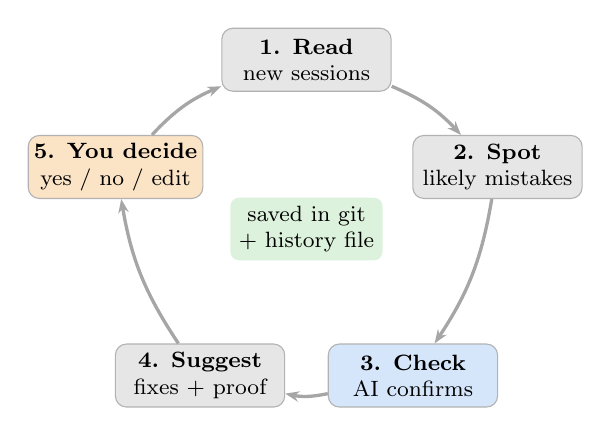
\begin{tikzpicture}[
  stp/.style={draw=gray!60,rounded corners=4pt,align=center,font=\footnotesize,minimum width=2.15cm,minimum height=0.8cm,inner sep=2pt},
  arr/.style={-{Stealth[length=5pt]},very thick,gray!70}]
\node[stp,fill=code]  (read)   at (90:2.15)  {\textbf{1. Read}\\new sessions};
\node[stp,fill=code]  (spot)   at (18:2.55)  {\textbf{2. Spot}\\likely mistakes};
\node[stp,fill=ai]    (check)  at (-54:2.3) {\textbf{3. Check}\\AI confirms};
\node[stp,fill=code]  (suggest) at (-126:2.3) {\textbf{4. Suggest}\\fixes + proof};
\node[stp,fill=you]   (decide) at (162:2.55) {\textbf{5. You decide}\\yes / no / edit};
\node[font=\footnotesize,align=center,fill=saved,rounded corners=3pt,inner sep=3pt] at (0,0) {saved in git\\+ history file};
\draw[arr] (read) to[bend left=12] (spot);
\draw[arr] (spot) to[bend left=12] (check);
\draw[arr] (check) to[bend left=12] (suggest);
\draw[arr] (suggest) to[bend left=12] (decide);
\draw[arr] (decide) to[bend left=12] (read);
\end{tikzpicture}
\caption{One run. \chip{code}{grey: plain code} \chip{ai}{blue: AI} \chip{you}{orange: you}. The next run starts from what was saved.}
\end{figure}

\textbf{1. Read.} Load the sessions since the last run, remove secrets.

\textbf{2. Spot.} Simple checks run over every session, like a spell-checker for chats. Some mistakes are clear from the log alone (``the same command failed 3 times in a row''), so code decides those. Others are only likely (``the user wrote \emph{I told you}''), so code just marks the spot. The checks are tuned to miss as little as possible, because step 3 removes false alarms.

\textbf{3. Check.} For each marked spot, an AI gets the few lines around it and one question, for example ``did the user repeat a correction?''. It must answer in a fixed form: yes, no, or ``a different problem'' with a short note. The AI comes from a different company than the coding AI, since AI judges tend to go easier on their own family [6].

\begin{center}
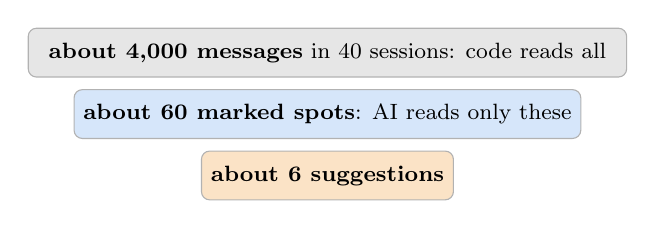
\begin{tikzpicture}[f/.style={draw=gray!60,rounded corners=3pt,align=center,font=\footnotesize,minimum height=0.62cm}]
\node[f,fill=code,minimum width=7.6cm] (a) at (0,0) {\textbf{about 4,000 messages} in 40 sessions: code reads all};
\node[f,fill=ai,minimum width=5.4cm] (b) at (0,-0.78) {\textbf{about 60 marked spots}: AI reads only these};
\node[f,fill=you,minimum width=3.2cm] (c) at (0,-1.56) {\textbf{about 6 suggestions}};
\end{tikzpicture}\\[-2pt]
{\scriptsize\itshape Typical sizes for one engineer. The AI reads a small slice, so it is cheaper and more accurate.}
\end{center}

\textbf{4. Suggest.} Count how often each mistake happened and in how many sessions. Only repeated mistakes become suggestions. Each one is placed where it belongs: a rule, a new agent, a new skill, a tool fix, or a habit tip [7].

\textbf{5. You decide.} Accept, reject or edit each item. Accepted ones are written to the files and committed. All choices, including rejections, are saved so the tool doesn't ask again.

\textbf{What it looks for at the start.} From the task brief, research on how AI agents fail [8], and Claude Code's similar \texttt{/insights} command [9]:

\vspace{2pt}
{\footnotesize
\begin{tabularx}{\columnwidth}{@{}>{\raggedright\arraybackslash}X >{\raggedright\arraybackslash}p{3.0cm}@{}}
\toprule
\textbf{What keeps happening} & \textbf{Suggested fix}\\
\midrule
Session runs too long, on many topics & tip: one session per task \\
Review done by the same agent that wrote the code & a separate reviewer agent \\
User repeats the same correction & one line in \texttt{AGENTS.md} \\
AI says ``done'' without running tests & rule: test before ``done'' \\
Same failing command, again and again & fix the tool or add a rule \\
Same steps done by hand in many sessions & a new skill for them [10] \\
Something new & added to this list \\
\bottomrule
\end{tabularx}}

\section{Using it}
\textbf{Step 1.} In opencode, type \texttt{/improve}. It takes a few minutes.

\textbf{Step 2.} Read the short report. Each item looks like this:

\begin{tcolorbox}[colback=white,colframe=gray!50,boxrule=0.5pt,arc=3pt,left=4pt,right=4pt,top=3pt,bottom=3pt,fontupper=\small]
\chip{saved}{New rule for \texttt{AGENTS.md}}\par\vspace{2pt}
\textbf{``Run the unit tests after your last edit, before saying done.''}\par\vspace{2pt}
Seen in \textbf{6 of 40} sessions. Example from Monday, 09:08:\par
{\ttfamily\scriptsize
\hspace*{6pt}agent: ran tests $\to$ 2 failed\\
\hspace*{6pt}agent: edited calc.ts\\
\hspace*{6pt}agent: ``Fixed the rounding. Done!''}\par\vspace{3pt}
\hfill\chip{saved}{accept}\ \chip{code}{reject}\ \chip{you}{edit}
\end{tcolorbox}

\textbf{Step 3.} Click accept, reject or edit. That's it.

\textbf{Why the report looks like this.} Research shows that long AI explanations make people accept advice whether it is right or not [11]. Proof only helps when checking it is quicker than trusting it [12]. So each item shows a count and the real log lines, which take seconds to check. The report talks about sessions, not about the person, since feedback aimed at the person often makes performance worse [13]. And it stays short: at Google, engineers ignored checking tools that raised too many false alarms (above about 10\%) [14].

\section{How it gets better over time}
\begin{itemize}
\item \textbf{Rules must earn their place.} Each rule remembers which mistake it should fix. If that mistake goes down over the next runs, the rule gets $+1$; if not, $-1$. A rule that keeps losing points is suggested for removal. This follows ExpeL, which keeps a list of lessons and votes them up or down [15], and ACE, which updates the AI's instructions in small steps instead of rewriting them [16]. \texttt{AGENTS.md} has a size limit; long rules for one kind of task move to a separate file it points to.
\item \textbf{New mistakes get added.} The ``a different problem'' notes from step 3, plus a few full sessions the AI reads each run, are collected. When the same kind of note keeps coming back, it is suggested as a new item for the list, together with a new check for step 2 that was tested on past sessions.
\item \textbf{Noisy checks are switched off.} If you keep rejecting what one check finds, it is muted until fixed.
\item \textbf{Nothing is forgotten.} A fixed mistake is still counted, so we see if it comes back, for example after switching AI models.
\end{itemize}

\noindent\begin{minipage}{\columnwidth}
\textbf{One run, in short:}
\begin{lstlisting}
sessions = clean(load_new_sessions())
spots    = run_checks(sessions)          # plain code
answers  = ai_confirm(spots)             # short pieces only
counts   = count_per_mistake(answers)
for item in suggest(counts, history):
    if engineer_accepts(item):
        apply_and_commit(item)
    history.save(item)                   # yes and no
\end{lstlisting}
\end{minipage}

\section{How I would test it}
\begin{figure}[h]
\centering
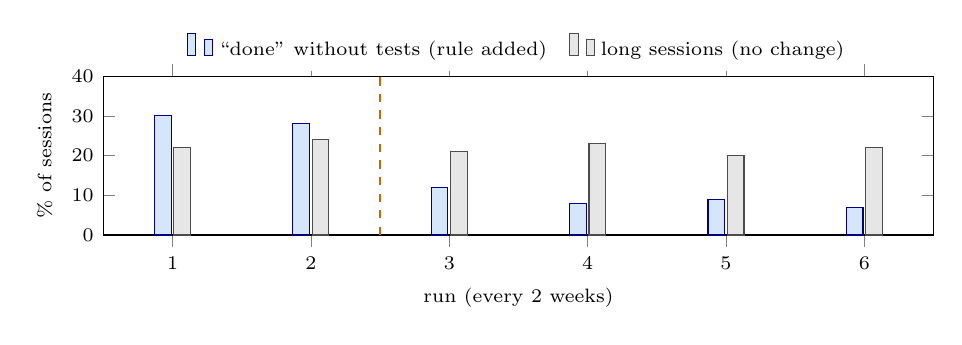
\begin{tikzpicture}
\begin{axis}[width=\columnwidth,height=3.6cm,ybar=1pt,bar width=6pt,
  ymin=0,ymax=40,ylabel={\% of sessions},ylabel style={font=\scriptsize},
  xtick={1,...,6},xlabel={run (every 2 weeks)},xlabel style={font=\scriptsize},
  tick label style={font=\scriptsize},legend style={font=\scriptsize,draw=none,at={(0.5,1.03)},anchor=south,legend columns=-1,/tikz/every even column/.append style={column sep=6pt}},
  legend cell align=left,enlarge x limits=0.1]
\addplot[fill=ai,draw=blue!50!black] coordinates {(1,30)(2,28)(3,12)(4,8)(5,9)(6,7)};
\addplot[fill=code,draw=gray!60!black] coordinates {(1,22)(2,24)(3,21)(4,23)(5,20)(6,22)};
\draw[dashed,thick,orange!80!black] (axis cs:2.5,0) -- (axis cs:2.5,40);
\legend{``done'' without tests (rule added),long sessions (no change)}
\end{axis}
\end{tikzpicture}
\caption{Example with made-up numbers. The rule was accepted after run 2. Only its mistake drops, so the drop is likely due to the rule and not to an easier month.}
\end{figure}
\begin{enumerate}
\item Read about 20 real sessions and mark every mistake by hand. Use 10 to build the checks and keep 10 aside for the final test.
\item The simple checks must find almost every marked mistake (over 90\%).
\item The AI must agree with my marks most of the time (a standard agreement score above 0.7; a similar study reached 0.77 [8]).
\item After a fix is accepted, its mistake should drop more than mistakes that were not touched (see the chart).
\item Repeat steps 2 and 3 whenever the AI model or the list changes.
\end{enumerate}

\section{Limits}
\begin{itemize}
\item It only sees what happens inside opencode.
\item One person's sessions give small numbers, so some answers will be ``not enough data yet''.
\item A drop after a fix is a good sign, not proof.
\item The AI can be wrong, and the simple checks miss wordings they were never shown.
\item A report nobody reads changes nothing, so it must stay short.
\end{itemize}

\section{Next steps}
\begin{itemize}
\item \textbf{Team version.} One anonymous line per session, grouped by topic, and a group is shown only if many engineers share it, as in Anthropic's Clio [17]. Secrets must be removed first, since such privacy layers can be attacked.
\item \textbf{Live tips} inside opencode, e.g.\ ``this session is getting long, start a new one?''.
\item \textbf{Skills that build on skills}, from steps that repeat across sessions [10].
\end{itemize}

\vspace{2pt}
\hrule
\vspace{3pt}
{\scriptsize
\textbf{A note on sources.} AI engineering changes every few months, so many good practices first appear in talks and videos by the people who build these tools, long before a paper (Claude Code's \texttt{/insights} [9] is mostly explained in posts and talks). Developers already learn this way: in the 2025 Stack Overflow survey, 60.5\% use YouTube for community, 70\% of those learning to code [18], and developers have long used YouTube to share know-how [19]. I also used a general AI engineering course on YouTube as a check; two of its points shaped this design: learn by building small things, and keep checking your system with an independent review [20].

\vspace{3pt}
\textbf{References.}
[1] Schluntz \& Zhang, \emph{Building effective agents}, Anthropic, 2024.
[2] Fortune, \emph{AI coding tool Replit wiped database, called it a catastrophic failure}, Jul 2025.
[3] Deshpande et al., \emph{TRAIL}, arXiv:2505.08638, 2025.
[4] Hong et al., \emph{Context Rot}, Chroma, 2025.
[5] Karpathy, \emph{Software Is Changing (Again)}, YC AI Startup School 2025, \href{https://youtube.com/watch?v=LCEmiRjPEtQ}{YouTube}.
[6] Pombal et al., \emph{Self-preference bias in rubric-based evaluation}, arXiv:2604.06996, 2026.
[7] \emph{Self-evolving agentic harnesses} (HarnessFix: ``localize before you fix''), 2026.
[8] Cemri et al., \emph{Why do multi-agent LLM systems fail?}, NeurIPS 2025.
[9] Claude Code \texttt{/insights} command, Anthropic, Feb 2026.
[10] Wang et al., \emph{Agent Workflow Memory}, ICML 2025.
[11] Bansal et al., \emph{Does the whole exceed its parts?}, CHI 2021.
[12] Vasconcelos et al., \emph{Explanations can reduce overreliance on AI}, CSCW 2023.
[13] Kluger \& DeNisi, \emph{The effects of feedback interventions on performance}, 1996.
[14] Sadowski et al., \emph{Lessons from building static analysis tools at Google}, CACM 2018.
[15] Zhao et al., \emph{ExpeL}, AAAI 2024.
[16] Zhang et al., \emph{Agentic Context Engineering}, ICLR 2026.
[17] Tamkin et al., \emph{Clio}, Anthropic, 2024.
[18] Stack Overflow Developer Survey 2025.
[19] MacLeod, \emph{Code, Camera, Action!: how developers share program knowledge using YouTube}, 2015.
[20] Simplilearn, \emph{AI Engineer Full Course 2026}, YouTube.
}

\end{document}
